\documentclass{article}
\usepackage[utf8]{inputenc}
\usepackage[T1]{fontenc}
\usepackage[french]{babel}
\usepackage{textcomp}
\usepackage{amsmath,amssymb,amsthm}
\usepackage{lmodern}
\usepackage[a4paper]{geometry}
\usepackage{graphicx}
\usepackage{xcolor}
\usepackage{multicol}
\usepackage{microtype}
\usepackage{pdfpages}
\usepackage{listings}
\usepackage{color}


\usepackage{hyperref}
\hypersetup{pdfstartview=XYZ}
 

\usepackage{fancyhdr}
\pagestyle{fancy}
\renewcommand\headrulewidth{0.4pt}
\fancyhead[L]{Le Cesne Benjamin - Tardy Luca}
\fancyhead[R]{Prep'ISIMA / L2 INFO}
\renewcommand\footrulewidth{0.4pt}
\fancyfoot[C]{
\textbf{Page \thepage/8}}
\fancyfoot[L]{\textit{Projet - Prep'ISIMA}}
\fancyfoot[R]{\today}

\newcommand{\variable}[1]{\texttt{#1}}
\newcommand{\code}[1]{\lstinputlisting{#1}}


\definecolor{darkWhite}{rgb}{0.92,0.92,0.92}

\lstset{frame=single,
  language=C,
  showstringspaces=false,
  columns=flexible,
  backgroundcolor=\color{darkWhite},
  basicstyle={\small\ttfamily},
  numbers=left,
  numberstyle=\tiny\color{black},
  framexleftmargin=20pt,
  framexrightmargin=20pt,
  keywordstyle=\color{blue},
  commentstyle=\color{red},
  stringstyle=\color{violet},
  breaklines=true,
  breakatwhitespace=true,
  tabsize=2,
  literate=
  {à}{{\`a }}1
  {é}{{\'e}}1
  {è}{{\`e}}1
  {ê}{{\^e}}1
  {ù}{{\`u}}1
  {î}{{\^i}}1
  {ç}{{\c{c}}}1
}


\begin {document}
\hfill
\hfill
\hfill
\begin{center}
  \large{PROJET EULER}

  Problème 117
\end{center}
\tableofcontents
\newpage
\part {Résolution du problème}
\section {Présentation}

Le principe de ce problème est de remplir un certain nombre de cases avec des rectangles plus ou moins long. Les bleus mesurent 4 de long, les vert 3 et les rouge 2. Une dernière contrainte est imposée : l'ordre compte.
\newline Prenons 4 cases vides. \, 
\includegraphics[scale = 0.2]{Images/vide.png} \, On peut choisir de les remplir par "rien". Déjà une possibilité. On peut maintenant choisir de mettre un bleu : \, 
\includegraphics[scale = 0.2]{Images/bleu.png} \,. Il mesure 4, il prend ainsi toute la place. On veut maintenant placer des verts. On peut les placer de deux manières différentes : \, 
\includegraphics[scale = 0.2]{Images/vert1.png} \, ou \, 
\includegraphics[scale = 0.2]{Images/vert2.png} \,. Enfin, il faut placer les rouges. Il y a bien évidement ces dispositions : \, 
\includegraphics[scale = 0.2]{Images/rouge1.png} \, et \, 
\includegraphics[scale = 0.2]{Images/rouge2.png} \,. On remarque que l'on peut également mettre 2 rouges à la suite : \, 
\includegraphics[scale = 0.2]{Images/rouge3.png} \,. Mais étant donné que l'ordre des rectangles compte, la possibilité suivante est aussi bonne \, 
\includegraphics[scale = 0.2]{Images/rouge4.png} \,. On arrive donc à un bilan de 4 possibilités pour les rouges, 2 pour les verts, 1 pour les bleus et la possibilité vide. Il y a 8 façon de remplir 4 cases, en suivant les contraintes de ce problème.
\newline Pour donner un autre exemple, il y a 15 manières de remplir 5 cases :
\bigbreak
\begin{center}
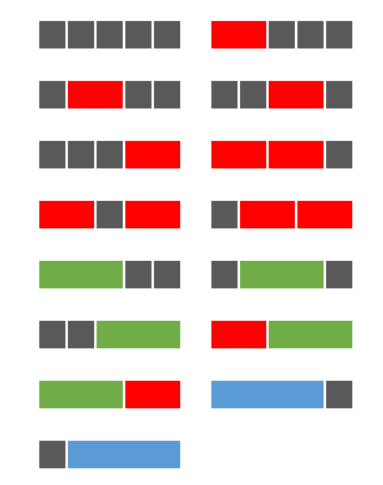
\includegraphics[scale = 0.5]{Images/presentation.png}
\end{center}
\bigbreak

Le but de problème est de déterminer combien il y a de possibilités de remplir 50 cases.
\newpage
\section{Méthodes de réflexion}

\subsection{Première méthode (méthode récursive)}

\subsubsection{Algorithme de principe}

Cet algorithme prend en entrée un entier $n$ (représentant le nombre de cases à remplir), et retourne le nombre de possibilité de remplir les n cases, en respectant les contraintes du problème. Il s'effectue de manière récursive. Pour exemple en rentrant 5, le programme renvoie 15.

\bigbreak
\lstinputlisting[language=bash]{Algo_de_principe/problem117_1_principe.txt}

\subsubsection{Développement}
Dans cette méthode récursive, nous considérons que pour remplir les 50 cases il faut déjà commencer par choisir comment remplir la première case. Il y a 4 réponses possibles à cette question : soit on ne la remplit pas, soit on pose un rectangle de 2 cases, soit de 3 cases ou soit de 4 cases. Dans le premier cas, il ne restera plus que 49 cases à remplir. Dans le deuxième cas, il n'en restera que 48, 47 dans le troisième et 46 dans le dernier. C'est pourquoi nous appelons la même fonction de façon récursive pour calculer le nombre de possibilités de remplir 49, 48, 47 et 46 cases. Ensuite on répète ce processus d'appel récursif sur les 4 précédents jusqu'à trouver un cas d'arrêt. Les cas d'arrêts sont au nombre de 4 avec cette méthode. En effet, on connaît gràce à l'exemple donné précédemment, le nombre de possibilités pour remplir 5 cases, donc 5 est un cas d'arrêt et on retourne 15 dans ce cas-là. Mais il est possible que l'on n'appelle jamais la fonction avec n = 5. En effet, lorsque n = 6, on appelle $recursive(5)$, $recursive(4)$, $recursive(3)$ et $recursive(2)$. Ainsi, 4, 3 et 2 sont des cas d'arrêts également.

Ceci correspond ainsi à une modélisation de la suite de Tetranacci, une dérivé de la suite de Fibonacci. En effet, si on appelle $F$ la suite de Fibonacci, on sait que $F(n) = F(n-1) + F(n-2)$. Ici, on remarque que $recursive(n) = recursive(n-1) + recursive(n-2) + recursive(n-3) + recursive(n-4)$. Ceci correspond à une suite où chaque terme est la somme des 4 précédents, la suite de tetranacci. Malheureusement, cette méthode est beaucoup trop longue, comme pour Fibonacci. En prenant 50 comme entrée, elle doit faire un nombre incalculable d'appels récursifs. Il faut donc la modifier pour ne plus faire appels à la fonction plusieurs fois avec la même entrée. En effet, ici, on appelle plusieurs fois la même fonction avec le même argument. Par exemple, en partant de 50, on l'appelle avec 49, 48, 47 et 46. Mais avec 49, on l'appelle encore avec 48, 47 et 46. Ceci n'est que le début, au total, le programme appelera $recursive(6)$ 1 965 381 541 064 de fois, pour donner un exemple. Il faut donc stocker le résultat de chaque appel pour ne plus avoir à le calculer.
\subsection{Seconde méthode (méthode tetranacci)}

\subsubsection{Algorithme de principe}

Cet algorithme prend en entrée un entier $n$ (représentant le nombre de cases à remplir), et retourne le nombre de possibilité de remplir les n cases, en respectant les contraintes du problème. Ici on stocke dans une liste les 4 précédents termes.
\bigbreak
\lstinputlisting[language=bash]{Algo_de_principe/problem117_2_principe.txt}

\subsubsection{Développement}
Ici, on remarque que la suite de Tetranacci (que l'on appelera $T$) commence, comme Fibonacci, à 0. Ainsi, $T(0) = 1, T(1) = T(0), T(2) = T(0) + T(1) et T(3) = T(0) + T(1) + T(2)$. On sait que chaque terme est la somme des 4 précédents. Il faut donc stocker ces 4 termes pour ne pas avoir à les recalculer. On stocke donc dans une liste 4 valeurs. A l'initialisation, il ne doit y avoir que $T(0)$. Or, pour calculer $T(1)$, on doit avoir accès à 4 valeurs pour pouvoir calculer une somme. C'est pourquoi on initialise cette liste à $[0,0,0,T(0)]$. Ensuite, tant que nous n'avons pas $n+3$ valeurs dans la liste, on y ajoute le prochain terme en faisant la somme des 4 derniers termes. $T(n)$ sera le $n+3^{ème}$ terme puisque les 3 premiers ne font pas à proprement parler de la suite. Ainsi, on calcule $T(n)$ très rapidement, en ne calculant que $n$ sommes. $T(50) = 100808458960497$, il y a donc 100808458960497 possibilités de remplir les 50 cases avec des rectangles de longueur 4, 3 et 2.

\newpage
\part {Optimisation}
\section {Objectifs}

Après avoir résolu le problème nous nous sommes fixé de nouveau objectifs :

\noindent - Essayer d'obtenir un algorithme plus simple, qui pourrait également prendre moins de place mémoire.

\noindent - Améliorer la lisibilité et la compréhension de nos méthodes, et si nécessaire en refaire une autre.

\section{Méthode finale}

\subsection{Algorithme de principe}

Cet algorithme prend en entrée un entier $n$ (représentant le nombre de cases à remplir), et retourne le nombre de possibilité de remplir les n cases, en respectant les contraintes du problème. On reprend le même principe que l'algorithme précédent, mais on stocke les termes précédents dans des variables.
\bigbreak
\lstinputlisting[language=bash]{Algo_de_principe/problem117_3_principe.txt}

\subsection{Développement}
Cette méthode est identique à la précédente à une différence près. Cette différence permet de réduire l'utilisation de l'espace mémoire puisque plutôt que de réserver $n+3$ cases mémoires, on n'en réserve que 4 dans tous les cas. En effet, pour calculer $T(n)$, on n'a besoin que des 4 termes précédents. On peut donc n'utiliser que 4 variables qui correspondent aux 4 derniers termes calculés. Comme précédemment, 3 variables sont initialisés à 0, et la dernière correspond à $T(0)$, elle est donc initialisée à 1. Ensuite, on réalise $n$ fois la somme des 4 variables afin de calculer le prochain terme. Ce résultat est stocké dans la dernière variable et les 3 autres prennent la valeur du terme qui les suit. Après $n$ sommes, la 4ème variable est donc égale à $T(n)$, on peut donc la renvoyer.
\newpage
\part{Comparaison des trois méthodes}
\section{Comparaison en temps}
Afin de mettre en évidence les différences d'efficacité entre nos méthodes, nous avons réalisé des tests. La première méthode est très limitée. En effet, comme expliqué précédement, elle nécessite beaucoup d'appels. Quand on cherche à résoudre le problème avec comme entrée 36, le programme met 219 secondes à retourner le résultat. Elle n'est pas du tout efficace. Les 2 autres méthodes quant-à-elles sont réellement plus efficaces. En effet, pour tout nombre entré inférieur à 100 000, elles mettent moins d'une secondes à retourner le bon résultat. On priviligira donc ces deux méthodes.

\section{Compléxité}

Afin d'établir la compléxité des méthodes, nous avons établi un graphique des résultats obtenu grâce à la première méthode.

\bigbreak
\begin{center}
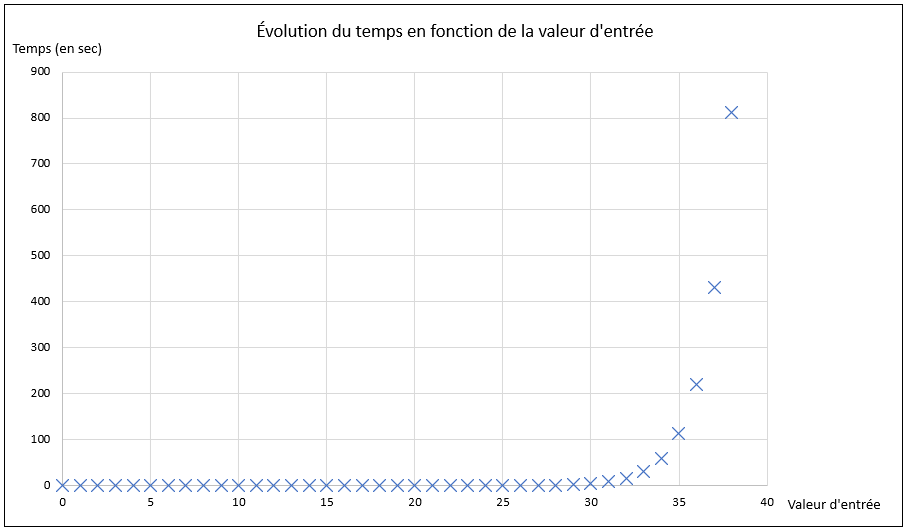
\includegraphics[scale = 0.5]{Images/graphique.png}
\end{center}
\bigbreak

On observe ainsi que la compléxité de cette méthode est exponentielle,$ O(e^n$). Cela s'explique par le nombre d'appel récursif effectué. On comprend pourquoi elle n'est pas du tout efficace comme méthode de résolution.

La compléxité des deux autres méthodes est linéaire, $O(n$), car on effectue $n$ fois les mêmes opérations.

On peut conclure qu'il est impensable d'utiliser la première méthode. Le choix d'utiliser la seconde ou la dernière méthode est en grande partie esthétique, même si la dernière utilise moins de place mémoire.

\newpage
\part{Annexes}
\section*{Méthode récursive}
\code{Algos/Problem117_1_rapport.py}


\section*{Méthode tetranacci}
\code{Algos/Problem117_2_rapport.py}

\newpage
\section*{Méthode finale}
\code{Algos/Problem117_3_rapport.py}

\end{document}
